\documentclass[english]{SPFShortReport}
\usepackage{subfigure}
\usepackage{longtable}
\usepackage[utf8]{inputenc}
\usepackage{url}
\usepackage{adjustbox}
\usepackage{gensymb}
\usepackage{booktabs}
\usepackage[yyyymmdd,hhmmss]{datetime}
\reportName{Type977 fitting for heat pump R410A}
\reportSubName{Parametric Heat Pump calculation} 
\reportDate{\today \hspace{0.1cm} at: \currenttime \hspace{0.1cm} h} 
\author{neha.dimri}
\address{neha.dimri}
\begin{document}
\begin{table}[!ht]
\centering
\caption{Fitted coefficients for the heat pump.}
\begin{adjustbox}{max width =\textwidth}
\begin{tabular}{l | c c } 
\hline
\hline
Coefficient &Description & \\ 
 & &$[kW]$\\ 
\hline
$P_{Q_{1}}$ & \emph{$1^{st}$ condenser polynomial coefficient}  & 1.3860e+01    \\ 
$P_{Q_{2}}$ & \emph{$2^{st}$ condenser polynomial coefficient}  & 1.2022e+02    \\ 
$P_{Q_{3}}$ & \emph{$3^{st}$ condenser polynomial coefficient}  & -7.9046e+00    \\ 
$P_{Q_{4}}$ & \emph{$4^{st}$ condenser polynomial coefficient}  & -1.6419e+02    \\ 
$P_{Q_{5}}$ & \emph{$5^{st}$ condenser polynomial coefficient}  & -1.7980e+01    \\ 
\hline
$P_{COP_{1}}$ & \emph{$1^{st}$ COP polynomial coefficient}  & 1.2490e+01    \\ 
$P_{COP_{2}}$ & \emph{$2^{st}$ COP polynomial coefficient}  & 6.4065e+01    \\ 
$P_{COP_{3}}$ & \emph{$3^{st}$ COP polynomial coefficient}  & -8.3022e+01    \\ 
$P_{COP_{4}}$ & \emph{$4^{st}$ COP polynomial coefficient}  & -2.3012e+02    \\ 
$P_{COP_{5}}$ & \emph{$5^{st}$ COP polynomial coefficient}  & 1.7321e+02    \\ 
\hline
$\dot m_{cond}$ & 10999296.00 $[kg/h]$ \\ 
$\dot m_{evap}$ & 10316127.60 $[kg/h]$ \\ 
\hline
$COP_{nom}$ (A0W35)& 4.70 \\ 
$Q_{cond,nom}$ (A0W35)& 12.55 $[kW]$\\ 
$Q_{evap,nom}$ (A0W35)& 9.88 $[kW]$\\ 
$W_{comp,nom}$ (A0W35)& 2.67 $[kW]$\\ 
\hline
 $RMS_{COP}$ & $4.83e-02$ \\ 
 $RMS_{Q_{cond}}$ & $1.16e-01$ \\ 
 $RMS_{W_{comp}}$ & $4.77e-02$ \\ 
\hline
Fit model & Inlet/Outlet Temperature\\ 
\hline
\hline
\end{tabular}
\end{adjustbox}
\label{CoefTable}
\end{table}
\begin{table}[!ht]
\centering
\caption{Differences between experiments and fitted data for the heat pump.          $error=100 \cdot |\frac{Q_{exp}-Q_{num}}{Q_{exp}}|$ and $RMS = \sqrt { \sum{\frac{(Q_{exp}-Q_{num})^2}{n_p}} }$ where $n_p$ is the number of data points.}
\begin{adjustbox}{max width =\textwidth}
\begin{tabular}{l | c c c c c c c c c c } 
\hline
\hline
$T_{cond,out}$ &$T_{evap,in}$ &$COP$ &$COP_{exp}$ &error &$Q_{cond}$ &$Q_{cond,exp}$ &error &$W_{comp}$ &$W_{comp,exp}$ &error \\ 
$^oC$ &$^oC$ &$[-]$ &$[-]$ &$[\%]$ &$[kW]$ &$[kW]$ &$[\%]$ &$[kW]$ &$[kW]$ &$[\%]$\\ 
\hline
55.00  & -4.00 & 2.54 & 2.53 & 0.2 & 10.26 & 10.40 & 1.3 & 4.05 & 4.11 & 1.54\\ 
50.00  & -4.00 & 2.78 & 2.85 & 2.6 & 10.49 & 10.60 & 1.0 & 3.78 & 3.72 & 1.64\\ 
45.00  & -4.00 & 3.13 & 3.21 & 2.5 & 10.71 & 10.82 & 1.1 & 3.42 & 3.37 & 1.46\\ 
40.00  & -4.00 & 3.60 & 3.65 & 1.3 & 10.91 & 11.02 & 1.0 & 3.03 & 3.02 & 0.32\\ 
35.00  & -4.00 & 4.19 & 4.20 & 0.3 & 11.10 & 11.24 & 1.2 & 2.65 & 2.68 & 0.99\\ 
30.00  & -4.00 & 4.89 & 4.91 & 0.4 & 11.28 & 11.45 & 1.5 & 2.31 & 2.33 & 1.15\\ 
55.00  & -2.00 & 2.67 & 2.67 & 0.2 & 10.90 & 10.93 & 0.3 & 4.09 & 4.09 & 0.10\\ 
50.00  & -2.00 & 2.94 & 3.00 & 2.1 & 11.15 & 11.15 & 0.0 & 3.80 & 3.72 & 2.20\\ 
45.00  & -2.00 & 3.32 & 3.37 & 1.4 & 11.39 & 11.39 & 0.0 & 3.43 & 3.38 & 1.43\\ 
40.00  & -2.00 & 3.82 & 3.82 & 0.1 & 11.61 & 11.63 & 0.1 & 3.04 & 3.04 & 0.25\\ 
35.00  & -2.00 & 4.44 & 4.41 & 0.7 & 11.83 & 11.87 & 0.4 & 2.66 & 2.69 & 1.10\\ 
30.00  & -2.00 & 5.18 & 5.19 & 0.3 & 12.03 & 12.09 & 0.5 & 2.32 & 2.33 & 0.27\\ 
60.00  & 0.00 & 2.61 & 2.52 & 3.6 & 11.26 & 11.26 & 0.0 & 4.31 & 4.47 & 3.50\\ 
55.00  & 0.00 & 2.80 & 2.80 & 0.2 & 11.54 & 11.50 & 0.3 & 4.13 & 4.11 & 0.51\\ 
50.00  & 0.00 & 3.10 & 3.14 & 1.4 & 11.81 & 11.76 & 0.4 & 3.81 & 3.75 & 1.85\\ 
45.00  & 0.00 & 3.51 & 3.52 & 0.2 & 12.07 & 12.01 & 0.5 & 3.44 & 3.41 & 0.69\\ 
40.00  & 0.00 & 4.05 & 4.03 & 0.4 & 12.32 & 12.51 & 1.5 & 3.04 & 3.10 & 1.94\\ 
35.00  & 0.00 & 4.70 & 4.64 & 1.2 & 12.55 & 12.74 & 1.5 & 2.67 & 2.75 & 2.64\\ 
30.00  & 0.00 & 5.46 & 5.46 & 0.0 & 12.78 & 12.26 & 4.2 & 2.34 & 2.25 & 4.19\\ 
60.00  & 2.00 & 2.71 & 2.62 & 3.4 & 11.87 & 11.83 & 0.4 & 4.38 & 4.52 & 2.96\\ 
55.00  & 2.00 & 2.93 & 2.92 & 0.2 & 12.18 & 12.10 & 0.6 & 4.16 & 4.14 & 0.46\\ 
50.00  & 2.00 & 3.26 & 3.26 & 0.1 & 12.47 & 12.37 & 0.8 & 3.83 & 3.79 & 0.91\\ 
45.00  & 2.00 & 3.70 & 3.70 & 0.1 & 12.75 & 12.64 & 0.9 & 3.44 & 3.42 & 0.76\\ 
40.00  & 2.00 & 4.27 & 4.22 & 1.2 & 13.02 & 12.92 & 0.8 & 3.05 & 3.06 & 0.37\\ 
35.00  & 2.00 & 4.95 & 4.88 & 1.4 & 13.28 & 13.19 & 0.7 & 2.68 & 2.70 & 0.73\\ 
30.00  & 2.00 & 5.74 & 5.73 & 0.3 & 13.52 & 13.46 & 0.5 & 2.35 & 2.35 & 0.21\\ 
60.00  & 4.00 & 2.81 & 2.76 & 1.8 & 12.49 & 12.45 & 0.3 & 4.45 & 4.51 & 1.42\\ 
55.00  & 4.00 & 3.06 & 3.06 & 0.2 & 12.82 & 12.73 & 0.7 & 4.19 & 4.16 & 0.84\\ 
50.00  & 4.00 & 3.42 & 3.44 & 0.6 & 13.13 & 13.02 & 0.9 & 3.84 & 3.78 & 1.51\\ 
45.00  & 4.00 & 3.90 & 3.87 & 0.7 & 13.43 & 13.33 & 0.8 & 3.45 & 3.44 & 0.10\\ 
40.00  & 4.00 & 4.49 & 4.43 & 1.4 & 13.73 & 13.61 & 0.8 & 3.06 & 3.07 & 0.52\\ 
35.00  & 4.00 & 5.20 & 5.12 & 1.6 & 14.00 & 13.91 & 0.7 & 2.69 & 2.72 & 0.91\\ 
30.00  & 4.00 & 6.03 & 6.04 & 0.2 & 14.27 & 14.20 & 0.5 & 2.37 & 2.35 & 0.69\\ 
60.00  & 6.00 & 2.91 & 2.88 & 1.0 & 13.10 & 13.10 & 0.0 & 4.51 & 4.55 & 0.91\\ 
55.00  & 6.00 & 3.18 & 3.21 & 0.8 & 13.45 & 13.39 & 0.5 & 4.22 & 4.17 & 1.27\\ 
50.00  & 6.00 & 3.58 & 3.61 & 0.9 & 13.79 & 13.70 & 0.7 & 3.85 & 3.80 & 1.56\\ 
45.00  & 6.00 & 4.09 & 4.06 & 0.7 & 14.12 & 14.03 & 0.6 & 3.45 & 3.46 & 0.07\\ 
40.00  & 6.00 & 4.71 & 4.64 & 1.6 & 14.43 & 14.34 & 0.6 & 3.06 & 3.09 & 0.94\\ 
35.00  & 6.00 & 5.46 & 5.40 & 1.0 & 14.73 & 14.67 & 0.4 & 2.70 & 2.72 & 0.60\\ 
30.00  & 6.00 & 6.31 & 6.35 & 0.6 & 15.02 & 14.98 & 0.3 & 2.38 & 2.36 & 0.86\\ 
60.00  & 8.00 & 3.01 & 3.02 & 0.4 & 13.72 & 13.75 & 0.2 & 4.56 & 4.55 & 0.24\\ 
55.00  & 8.00 & 3.31 & 3.35 & 1.1 & 14.09 & 14.10 & 0.1 & 4.25 & 4.21 & 1.01\\ 
50.00  & 8.00 & 3.74 & 3.78 & 1.1 & 14.45 & 14.45 & 0.0 & 3.87 & 3.82 & 1.11\\ 
45.00  & 8.00 & 4.28 & 4.25 & 0.7 & 14.80 & 14.78 & 0.1 & 3.46 & 3.48 & 0.56\\ 
40.00  & 8.00 & 4.94 & 4.88 & 1.1 & 15.13 & 15.13 & 0.0 & 3.07 & 3.10 & 1.10\\ 
35.00  & 8.00 & 5.71 & 5.66 & 0.9 & 15.46 & 15.48 & 0.1 & 2.71 & 2.73 & 0.99\\ 
30.00  & 8.00 & 6.60 & 6.68 & 1.2 & 15.77 & 15.82 & 0.3 & 2.39 & 2.37 & 0.93\\ 
60.00  & 10.00 & 3.11 & 3.14 & 1.1 & 14.34 & 14.47 & 0.9 & 4.62 & 4.61 & 0.18\\ 
55.00  & 10.00 & 3.44 & 3.51 & 1.9 & 14.73 & 14.83 & 0.7 & 4.28 & 4.23 & 1.22\\ 
50.00  & 10.00 & 3.90 & 3.94 & 1.0 & 15.11 & 15.21 & 0.6 & 3.88 & 3.86 & 0.38\\ 
45.00  & 10.00 & 4.47 & 4.48 & 0.2 & 15.48 & 15.59 & 0.7 & 3.46 & 3.48 & 0.50\\ 
40.00  & 10.00 & 5.16 & 5.12 & 0.7 & 15.84 & 15.95 & 0.7 & 3.07 & 3.12 & 1.44\\ 
35.00  & 10.00 & 5.96 & 5.95 & 0.2 & 16.18 & 16.35 & 1.0 & 2.71 & 2.75 & 1.21\\ 
30.00  & 10.00 & 6.88 & 7.03 & 2.1 & 16.52 & 16.70 & 1.1 & 2.40 & 2.38 & 1.04\\ 
\hline 
 Sum &  & &  & 52.4 &  &  & 36.1 & &  & 58.25\\ 
\hline 
 $RMS_{COP}$ & $4.83e-02$ \\ 
 $RMS_{Q_{cond}}$ & $1.16e-01$ \\ 
 $RMS_{W_{comp}}$ & $4.77e-02$ \\ 
\hline
\hline
\end{tabular}
\end{adjustbox}
\label{ErrorsTable}
\end{table}
\begin{figure}[!htbp]
\begin{center}
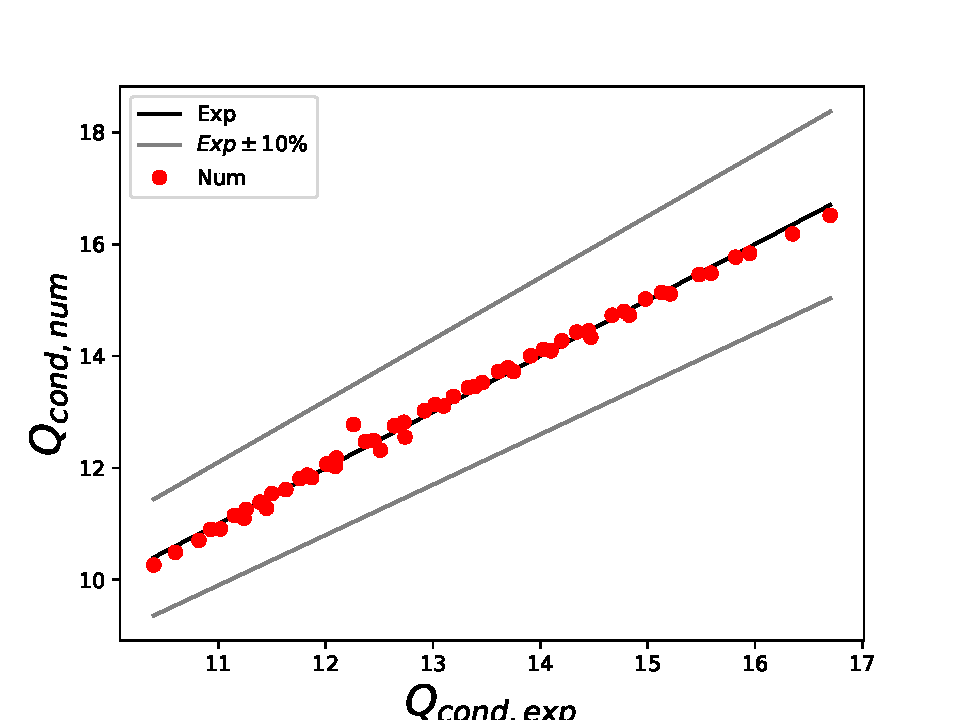
\includegraphics[width=1\textwidth]{C:/Daten/OngoingProject/OptimEase/HeatPumpFit/R410A/R410A-Qcond.pdf}
\caption{$Q_{cond}$ differences between experiments and fitted data}
\label{QcongFig}
\end{center}
\end{figure}
\begin{figure}[!htbp]
\begin{center}
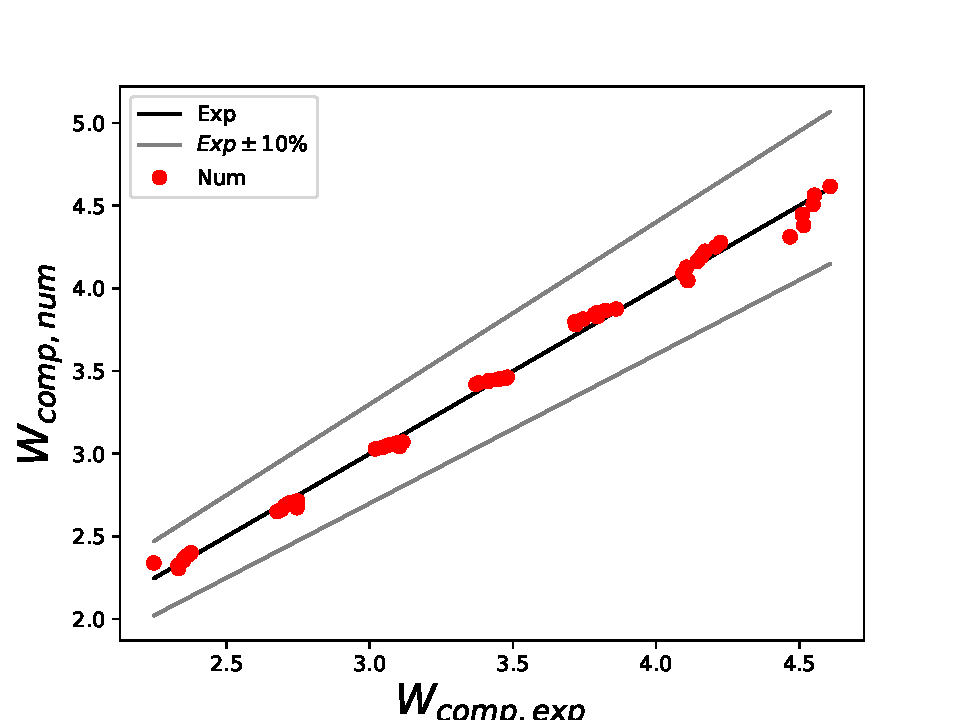
\includegraphics[width=1\textwidth]{C:/Daten/OngoingProject/OptimEase/HeatPumpFit/R410A/R410A-Qcomp.pdf}
\caption{$W_{comp}$ differences between experiments and fitted data}
\label{QcompFig}
\end{center}
\end{figure}
\begin{figure}[!htbp]
\begin{center}
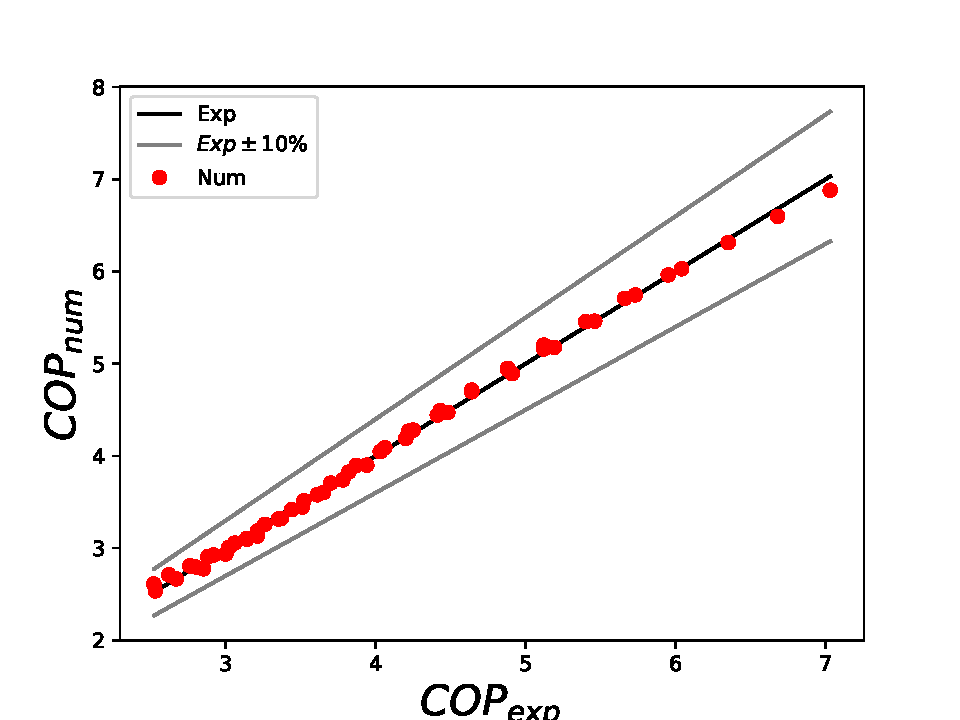
\includegraphics[width=1\textwidth]{C:/Daten/OngoingProject/OptimEase/HeatPumpFit/R410A/R410A-COP.pdf}
\caption{$COP$ differences between experiments and fitted data}
\label{COPFig}
\end{center}
\end{figure}
\end{document}
